% First, we share the results for house prices. Next, we present the results for employment and wages outcome variables.

\subsection{Road Maintenance}

\subsection{Road Quality decline}

 To assess the impact of cutting local road taxes on road quality, we utilized a fine-tuned Vision Transformer (ViT) model, leveraging labeled satellite imagery data for U.S. roads. The ViT model, fine-tuned using a large dataset of road images, assigned quality ratings on a scale of 0 (poor) to 2 (high) to our collected satellite imagery for Ohio neighborhoods, as explained in Section \ref{sec:road_quality}. We compared road quality ratings from the fine-tuned ViT model before and after the referendum in areas that failed to renew their road tax levy versus those that successfully passed the levy. These results are visually summarized in Figure \ref{fig:road_quality_change}, which shows the change in road quality ratings for both groups. 


\begin{figure}[htbp]
    \centering
    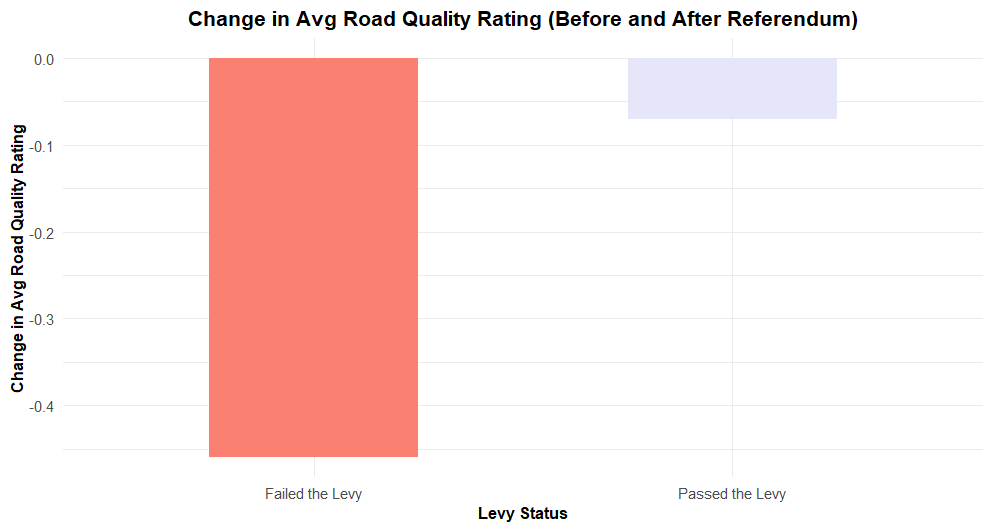
\includegraphics[width=\textwidth,keepaspectratio]{images/road_quality_change.png}
    \caption{Change in Road Quality Ratings Before and After Referendum}
    \label{fig:road_quality_change}
\end{figure}

Areas that failed to renew their tax levy experienced an average decline in road quality ratings of -0.5 points, equivalent to a 17\% deterioration in road quality relative to the three-point scale. In contrast, areas that maintained their tax levies saw a negligible decline of -0.08 points, suggesting effectively no deterioration in road quality. In neighborhoods where renewal taxes were cut, the decline in road quality highlights the potential long-term implications of fiscal policy decisions on public infrastructure maintenance.

\subsection{House Prices decline}

 Table \ref{tab:median_sale_amount} below shows the ITT estimates of failing a road tax levy on housing sale prices starting four years after the vote. 

 \begin{table}[ht]
    \centering
    \caption{Effect on median house prices of failing to renew a road tax levy}
    \label{tab:median_sale_amount}
    \begin{tabular}{p{2cm}ccccccc}
        \hline
        Year relative to vote & $t + 4$ & $t + 5$ & $t + 6$ & $t + 7$ & $t + 8$ & $t + 9$ & $t + 10$ \\
        \hline
        Treatment effect & -21,684 & -22,415 & -17,539 & -16,001 & -21,973 & -19,890 & -16,042 \\
        Standard error   & (7,838) & (8,348) & (8,465) & (6,918) & (9,111) & (7,756) & (8,915) \\
        Effective bandwidth ($h$) & 8.508 & 10.573 & 9.613 & 13.390 & 8.240 & 7.233 & 6.404 \\
        Bias bandwidth ($b$) & 16.430 & 19.894 & 17.133 & 23.953 & 15.327 & 14.073 & 16.469 \\
        Effective Observations & 469 & 605 & 525 & 801 & 402 & 324 & 260 \\
        Total Observations & 2,614 & 2,531 & 2,438 & 2,324 & 2,199 & 2,115 & 2,017 \\
        \hline
    \end{tabular}
    \begin{tablenotes}
        \small
        \item Outcome is median house price in constant 2010 U.S. dollars. Unit of observation is the city-year, so a treatment effect of -\$21,684 means that four years after the vote, cities that failed to renew road taxes and its associated spending have houses that sell for \$21,684 less than cities that vote to renew road taxes and spending. Treatment effects for years prior to $t + 4$ are statistically insignificant at the 5\% level; full results shown in Table \ref{tab:median_sale_amount_full}. The regressions include covariates related to the demographics and socioeconomic factors of the cities, drawn from Table \ref{tab:variable_means_sd}.
    \end{tablenotes}
\end{table}


Each treatment effect estimate represents the discount in median sale price for cities that cut road taxes in the years after voting on a road tax levy relative to otherwise similar cities that renew the taxes. Treatment effect estimates for years 4 through 9 after the vote are statistically significant in Table \ref{tab:median_sale_amount} as the $p$-values are below the canonical 0.05 threshold. The estimate for year $t + 10$ has a smaller estimate and is only significant at the 10\% level, suggesting that the effect of tax and service cuts on house prices may peter out ten years after the vote. Overall, we find an average reduction of \$15,349 in median house price over the 10 year period for houses in cities that vote to cut road tax levies representing 9\% of overall home value.\footnote{The average treatment effect estimate of \$15,349 was divided by the mean home sale price in the dataset of \$166,000 to get 9\%.}

\begin{figure}[htbp]
    \centering
    % 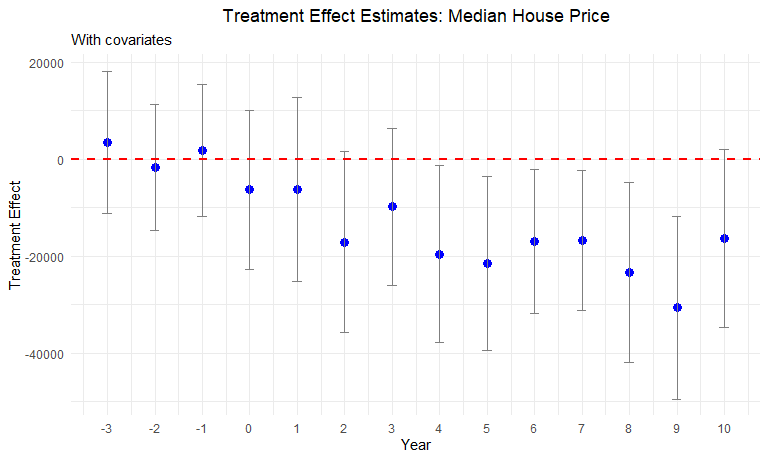
\includegraphics[width=\textwidth,keepaspectratio]{images/tes_gs.png}
    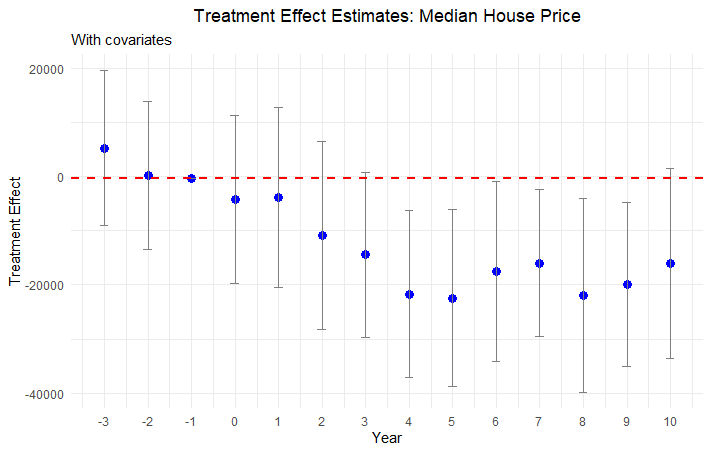
\includegraphics[width=\textwidth,keepaspectratio]{images/tes_gs_reg.png}    
    \caption{Effect plot for Median Housing Price}
    \label{fig:tes_hp}
\end{figure}

Figure \ref{fig:tes_hp} provides an event-study plot that summarizes the treatment effects for each time period. In the graph, we include placebo years up to 3 years before the treatment to show that the median housing prices are statistically identical for cities above and below the threshold prior to the treatment. Each blue dot represents the treatment effect estimate for that year and the bar around it represents the 95\% confidence interval for that estimate. For year 0, which is the year of the vote, we see a slight decrease in the estimate. However, this effect is not statistically significant, as evidenced by the confidence interval containing the null effect. Up to year 3, we observe that the treatment effect estimates are fairly close to zero, and the confidence interval overlaps with zero. As stated previously and shown in Table \ref{tab:median_sale_amount}, we start to see a sizable increase in treatment effect from year 4 onwards and continue to observe it through year 9 after the vote. 
 
\subsection{Heterogeneity Analysis} 

We show the results of our heterogeneity analysis, where we explore the differential impact of cutting road maintenance spending on house prices based on urban vs rural neighborhoods, the size of the tax levy and housing price quantiles.

\vskip 0.5cm

\textbf{Urban vs Rural neighborhoods}: We perform heterogeneity analysis to assess whether different types of neighborhoods and differing size of tax levies result in a differential impact on the housing prices. We first compare urban and rural areas in Ohio. We consider two different ways to define a city as urban:  one including only urbanized areas and another one including both urban areas and urbanized clusters. The event study plot in Figure 6 shows this result. 

\begin{figure}[htbp]
    \centering
    % 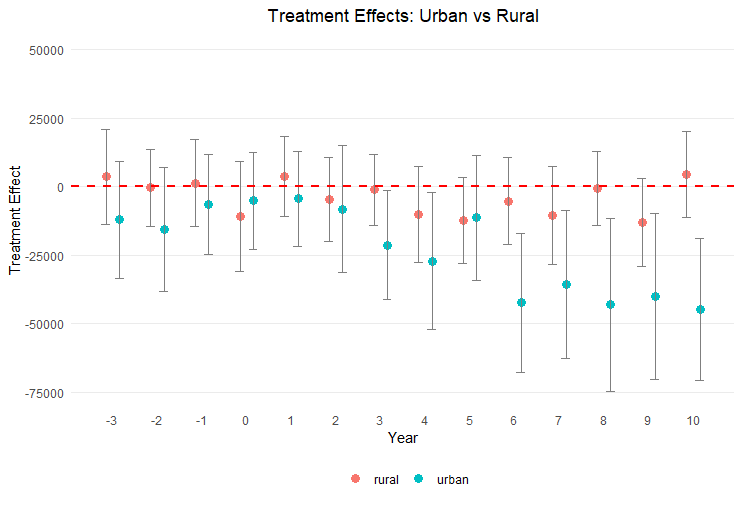
\includegraphics[width=\textwidth,keepaspectratio]{images/tes_covs_ua_new.png}
    % 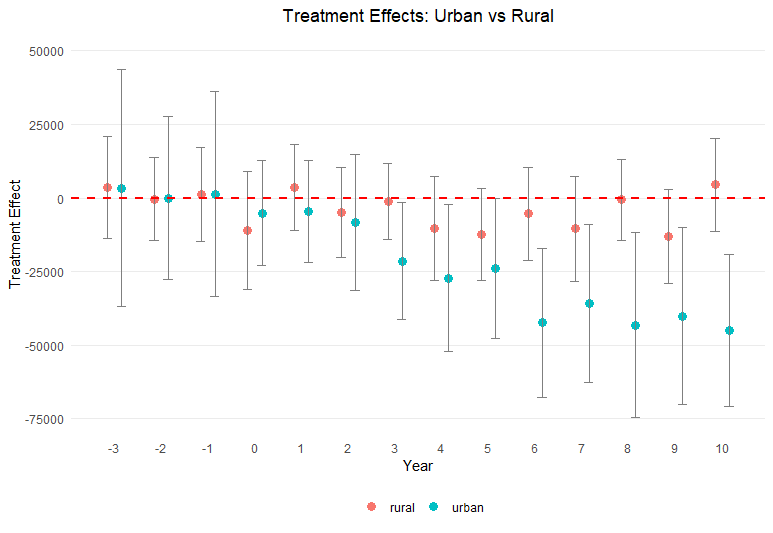
\includegraphics[width=\textwidth,keepaspectratio]{images/tes_covs_ua_clean.png}    
    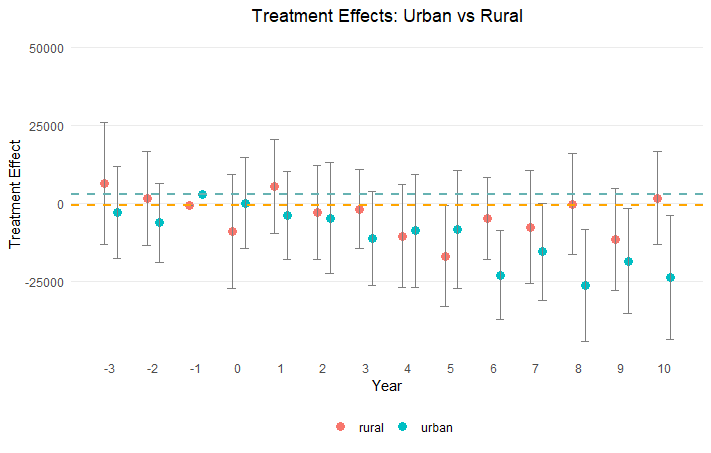
\includegraphics[width=\textwidth,keepaspectratio]{images/tes_covs_ua_reg.png}        
    \caption{Median Housing Price in Urban and Rural Areas}
    \label{fig:tes_covs_ua}
\end{figure}

As shown by Figure \ref{fig:tes_covs_ua}, we do not find any significant differences in housing prices after a renewal tax levy fails to pass for rural areas. On the other hand, we do find a statistically significant decline in housing prices in urban areas starting six years after voting. The standard errors are somewhat smaller for the rural estimates due to a larger number of observations. The difference in point estimates between urban and rural areas may stem from differences in housing supply elasticity (Brasington 2002). Overall, we find that housing prices decrease by \$25,825 on average over the decade after cutting road maintenance tax levies in urban areas. 

\vskip 1cm

\textbf{Tax magnitude}: We check whether the treatment effect is greater for bigger tax levies than smaller tax levies. For this analysis, we split the tax levies based on the millage of a tax levy that is voted upon, where one mill is one tenth of one percent. Mean millage in our dataset is 1.9. We split the data into two parts: small tax levies $\le$ 1.9 mills and large tax levies $>$ 1.9 mills. We do not identify a consistent statistically significant difference in treatment effects between smaller and larger tax levies, suggesting a lack of dose-response. Figure \ref{fig:tes_covs_size} illustrates this result.

\begin{figure}[htbp]
    \centering
    % 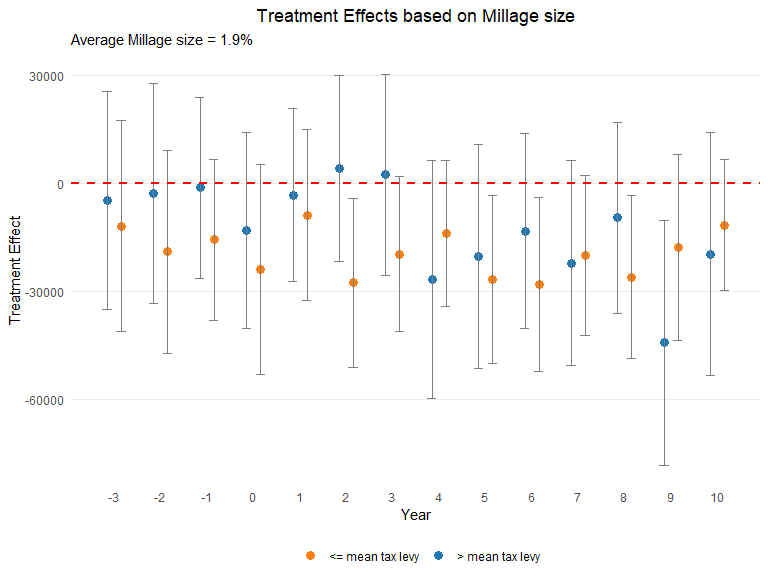
\includegraphics[width=\textwidth,keepaspectratio]{images/tes_size.png}
    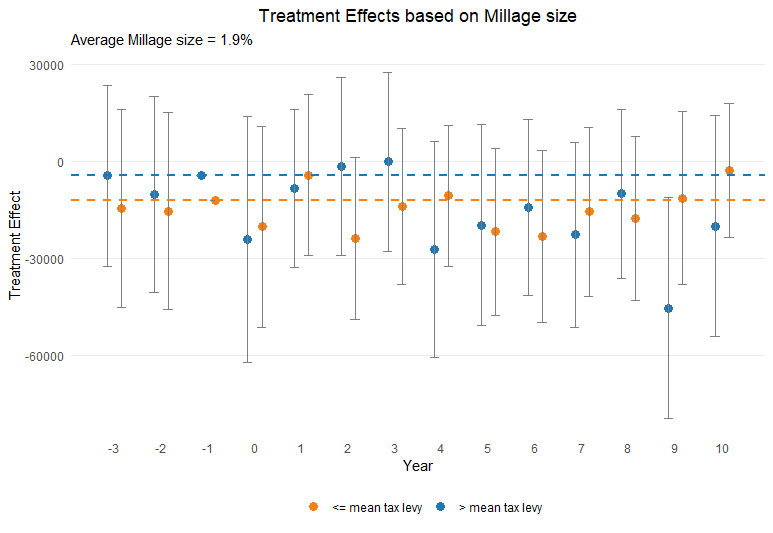
\includegraphics[width=\textwidth,keepaspectratio]{images/tes_size_re.png}    
    \caption{Median Housing Price based on Millage size}
    \label{fig:tes_covs_size}
\end{figure}

All the years before the reduction in road spending have treatment effect estimates with confidence intervals containing zero. Starting in year $t+2$, we observe statistically significant treatment effects in some years after the vote such as year 5, 6 and 8 that show a for tax levies with millage size equal to or below the mean. However, we do not see a consistent decrease in housing prices. Hence, we conclude that the decrease in housing prices of cities that fail to maintain their roads does not vary significantly based on the size of the tax levy.

\vskip 1cm

\textbf{RDD Quantile Estimation}: We further analyze our results by estimating quantile-level treatment effects, as suggested by Frandsen et al (2012), to study how the treatment’s impact varies at different quantiles of the outcome variable. 

\begin{table}[ht]
    \hspace{-1cm}
    % \centering
    \caption{Quantile-level Treatment Effects of Cutting Road Spending on Median House Prices}
    \label{tab:quantile_tes}
    \begin{tabular}{p{1.5cm}ccccccc}
        \hline
        Percentile & $t + 4$ & $t + 5$ & $t + 6$ & $t + 7$ & $t + 8$ & $t + 9$ & $t + 10$ \\
        \hline
        10\% & -6,433 & -22,570 & -9,602 & -12,984 & -11,217 & -6,569 & -1,326 \\
        & (9,364) & (9,065) & (9,205) & (8,420) & (9,136) & (10,809) & (8,793) \\
        20\% & -5,400 & -15,070 & 4,014 & -14,682 & -15,040 & -3,228 & 624 \\
        & (9,983) & (9,886) & (7,443) & (8,502) & (8,160) & (10,435) & (8,509) \\
        70\% & -21,760 & -11,171 & -38,082 & -36,685 & -21,356 & -25,605 & -18,600 \\
        & (12,333) & (11,806) & (12,835) & (12,163) & (12,218) & (13,984) & (9,872) \\
        80\% & -28,478 & -16,379 & -38,460 & -37,470 & -28,950 & -27,800 & -18,658 \\
        & (13,343) & (11,404) & (18,623) & (12,169) & (12,507) & (12,421) & (11,808) \\
        90\% & -51,470 & -34,604 & -38,510 & -27,039 & -29,010 & -49,093 & -36,662 \\
        & (18,409) & (15,837) & (22,194) & (16,308) & (16,640) & (14,498) & (19,110) \\
        \hline
    \end{tabular}
    \begin{tablenotes}
        \small
        \item The outcome is median house price in constant 2010 U.S. dollars. The unit of observation is the city-year, so a treatment effect of -\$28,478 means that at the 80th percentile of house prices four years after the vote, cities that fail to renew road taxes and its associated spending have houses that sell for \$28,478 less than cities that vote to renew road taxes and spending. The regressions include covariates related to the demographics and socioeconomic factors of the cities, drawn from Table \ref{tab:variable_means_sd}.
    \end{tablenotes}
\end{table}

\begin{figure}[htbp]
    \centering
    % 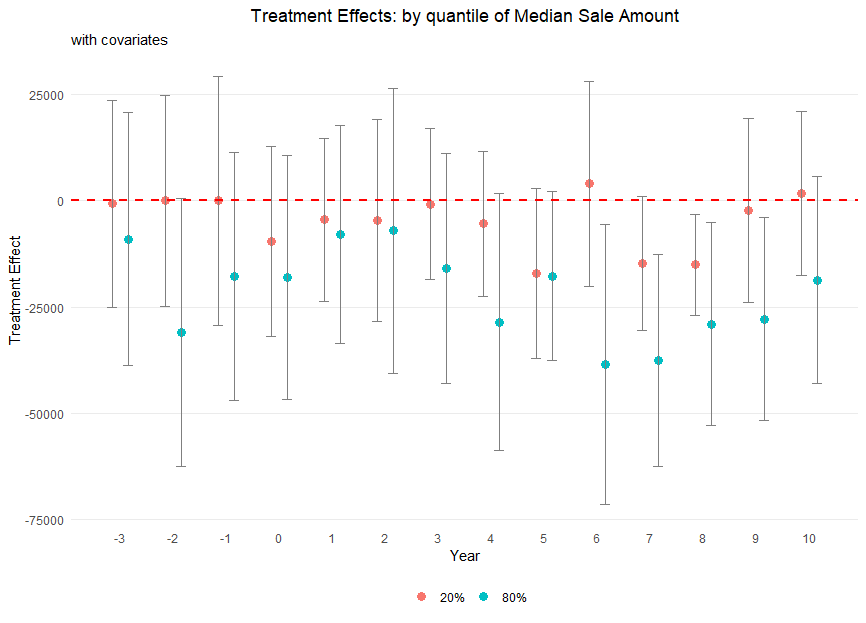
\includegraphics[width=\textwidth,keepaspectratio]{images/tes_qte_covs.png}
    % 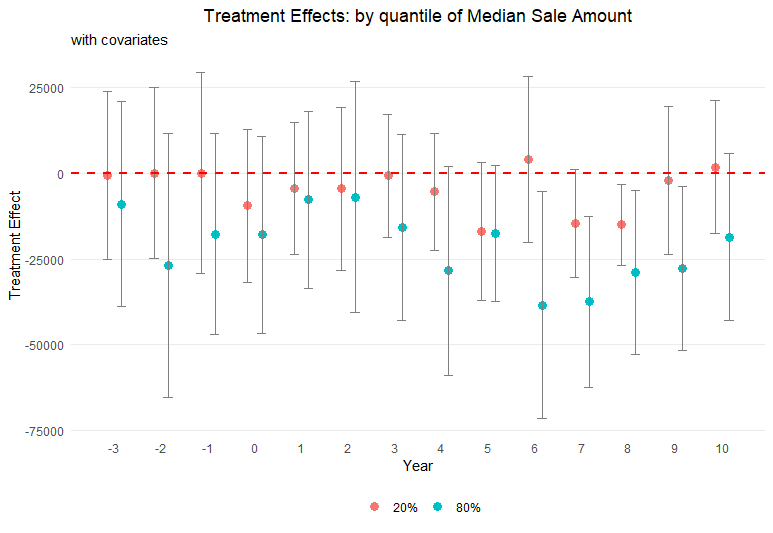
\includegraphics[width=\textwidth,keepaspectratio]{images/tes_qte.png}    
    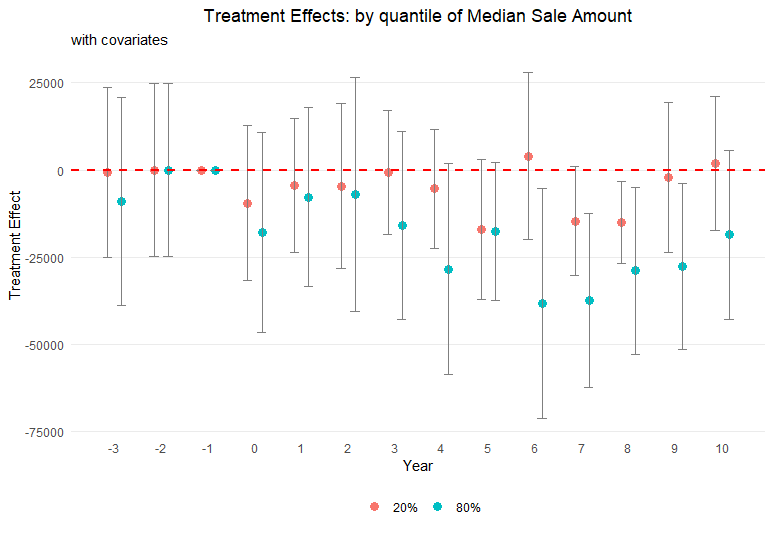
\includegraphics[width=\textwidth,keepaspectratio]{images/tes_qte_re.png}    
    \caption{Median Housing Price based on Quantiles: 20\% and 80\%}
    \label{fig:tes_qte_covs}
\end{figure}

Table \ref{tab:quantile_tes} shows the treatment effect heterogeneity of cutting road spending on high and low quantiles of median house prices. The top percentiles consistently exhibit a statistically significant decline in house sale prices, beginning in year 6 after the reduction in road spending. In contrast, the lower percentiles do not demonstrate a consistent treatment effect. This suggests a differential impact, where higher-valued properties are more sensitive to road disrepair than lower-valued houses. Figure \ref{fig:tes_qte_covs} contrasts the treatment effects of the 20th and 80th percentiles of home sale prices in an effect plot to highlight this differential impact of reduction in road maintenance spending.

\subsection{Robustness Tests}

We conduct several robustness tests to ensure the validity of our results. We test the sensitivity of our results to different bandwidths, covariates, and functional forms. We also check for the presence of pre-trends and perform a placebo test to confirm the validity of our RDD.

\vskip 0.5cm

\textbf{Removing contradictory observations}: In this test, we focus on ensuring the independence and exogeneity of our dataset, a critical aspect in assessing the impact of renewal tax levies on housing prices. An additional concern is the potential bias introduced by tax levies for additional money that might pass after renewal tax levy decisions.
To address this concern, we exclude observations from our analysis if a tax levy for additional funding is introduced and passed within a ten-year period following a renewal tax levy vote. This approach is premised on the notion that the introduction of new funding through additional levies could confound the effects of decreased road taxes on housing prices. 
For example, consider a scenario where a city votes on a renewal tax levy in the year 2000. If that city subsequently introduces and passes a tax levy for additional road spending in 2004, we exclude all votes for that city from 2005 through 2010. This exclusion ensures that the effect on house prices from the 2000 vote are captured for uncontaminated years but not for years after 2004 when the effect of additional road taxes may counteract the drop in tax money from the year 2000 vote. It allows us to isolate and examine the pure impact of the drop in funding from failing renewal levies on housing prices. 

\begin{table}[ht]
    \centering
    \caption{Effect on Median Sale Amount of Failing to Renew a Road Tax Levy}
    \label{tab:uncontaminated}
    \begin{tabular}{p{2.8cm}ccccccc}
        \hline
        year relative to vote & $t + 4$ & $t + 5$ & $t + 6$ & $t + 7$ & $t + 8$ & $t + 9$ & $t + 10$ \\
        \hline
        Treatment effect & -21,819 & -16,308 & -13,850 & -15,944 & -18,443 & -29,298 & -19,179 \\
        standard error & (11,271) & (7,489) & (8,161) & (8,186) & (8,591) & (8,342) & (10,120) \\
        Effective bandwidth (h) & 7.7 & 7.4 & 14.7 & 10.5 & 9.4 & 6.2 & 8.9 \\
        Bias bandwidth (b) & 13.6 & 17.8 & 24.5 & 19.0 & 18.4 & 13.3 & 18.2 \\
        Effective Observations & 538 & 512 & 1,086 & 680 & 584 & 347 & 492 \\
        Total Observations & 2,390 & 2,273 & 2,147 & 2,016 & 1,889 & 1,786 & 1,665 \\
        \hline
    \end{tabular}
    \begin{tablenotes}
        \small
        \item The outcome is median house price in constant 2010 U.S. dollars. The unit of observation is the city-year, so a treatment effect of -\$21,819 means that four years after the vote, cities that fail to renew road taxes and its associated spending have houses that sell for \$21,819 less than cities that vote to renew road taxes and spending. The regressions include covariates related to the demographics and socioeconomic factors of the cities, drawn from Table \ref{tab:variable_means_sd}.
    \end{tablenotes}
\end{table}

Upon implementing this data filtration, we observe that the treatment effect of the renewal levies on housing prices, measured from $t+1$ to $t+10$, remains largely consistent with our initial findings. This consistency in treatment effect, despite the exclusion of potentially confounding data, lends further credence to our results. The standard errors increase slightly due to reduction in sample size caused by the aforementioned data filtration process. 

\textbf{Placebo cutoffs}: In our primary analysis, the pivotal threshold for the vote share running variable is 50\%, indicating whether a renewal levy passes or fails.  Although we find significant treatment effects using this 50\% threshold, it could be random jumps in the data rather than cutting road taxes and funding that are responsible for the significant estimates.  To this end we conduct a series of placebo tests using alternative cutoffs: 30\%, 40\%, 60\%, and 70\%. Table \ref{tab:placebo_cutoffs} below summarizes the results from the placebo cutoffs analysis. 

\begin{table}[ht]
    \centering
    \caption{Robust Treatment Effect Estimate for Placebo Cutoffs}
    \label{tab:placebo_cutoffs}
    \begin{tabular}{p{2cm}cccc}
        \hline
        Years after vote & 30\% & 40\% & 60\% & 70\% \\
        \hline
        $t + 4$ & -2,540 & 7,037 & -4,037 & -43,670 \\
        & (8,473) & (6,993) & (10,961) & (21,452) \\
        $t + 5$ & -1,376 & -15,672 & -1,740 & 12,263 \\
        & (9,554) & (20,892) & (12,588) & (19,392) \\
        $t + 6$ & 10,589 & 9,476 & -13,479 & -617 \\
        & (8,894) & (7,721) & (13,661) & (18,438) \\
        $t + 7$ & 5,086 & 2,952 & -21,731 & -21,204 \\
        & (10,447) & (7,898) & (11,519) & (18,330) \\
        $t + 8$ & 9,900 & 11,821 & -11,014 & -37,686 \\
        & (10,745) & (8,241) & (12,460) & (15,717) \\
        $t + 9$ & 14,361 & 9,904 & -20,057 & -9,340 \\
        & (9,624) & (7,935) & (11,975) & (17,731) \\
        $t + 10$ & 12,147 & -25,540 & -13,828 & -16,358 \\
        & (13,649) & (31,460) & (10,267) & (21,396) \\
        \hline
    \end{tabular}
    \begin{tablenotes}
        \small
        \item Robust treatment effect estimate for placebo cutoffs as per the estimator from \cite{calonico2017rdrobust}. The unit of observation is city-year level. Standard errors are shown in parentheses below each estimate.
    \end{tablenotes}
\end{table}

Table \ref{tab:placebo_cutoffs} does not show consistently significant treatment effects for any of the placebo cutoffs for our parameter of interest. This absence of significance at thresholds other than the true 50\% reinforces the idea that the effects we observe at the 50\% mark are not a mere coincidence or a result of random variation in the data, but are indeed attributable to the dynamics surrounding the passing or failing of renewal tax levies. 

\textbf{Winsorization}: The debate over whether to include or exclude outliers continues, with some research suggesting that trimming outliers does not improve mean squared error (e.g., Bollinger and Chandra, 2005).  We now drop the 1\% tails to help curtail the influence of outliers. The overall sample mean after dropping 1\% tails is \$144,268 in constant 2010 dollars with a standard deviation of \$109,624. After performing this winsorization step, we re-estimate the treatment effect of failing to renew a road tax levy on housing outcome variables. The results from this estimation process are summarized in Figure \ref{fig:tes_g_w} below:

\begin{figure}[htbp]
    \centering
    % 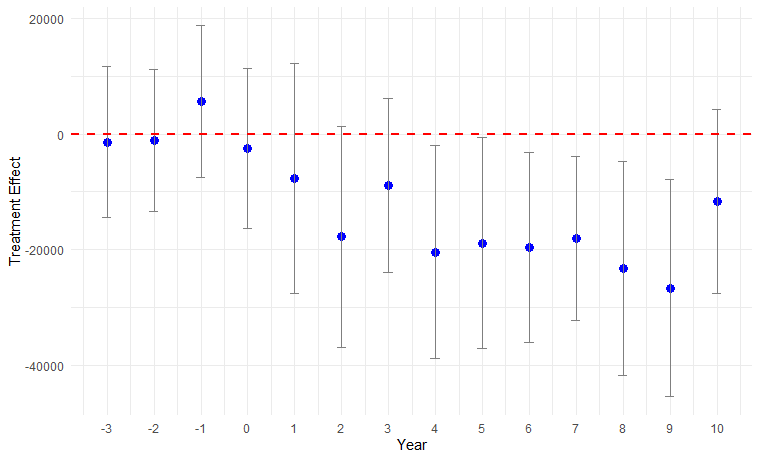
\includegraphics[width=\textwidth,keepaspectratio]{images/tes_g_w.png}
    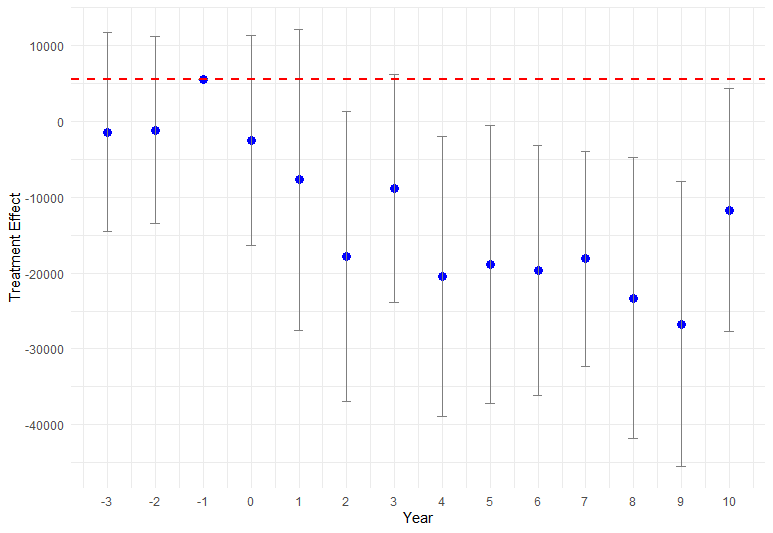
\includegraphics[width=\textwidth,keepaspectratio]{images/tes_g_w_re.png}    
    \caption{Median Housing Price after 1\% Winsorization}
    \label{fig:tes_g_w}
\end{figure}

The treatment effect estimates with winsorization mimic those from our baseline regression results qualitatively and quantitatively.

\section{Mechanisms} \label{sec:mech}

Initially, we discussed the limitations of road infrastructure papers, one of which is pinpointing a mechanism of action. \cite{currier2023} studies road roughness, finding an elasticity of speed with respect to road roughness between -0.14 and -0.30 depending on the methodology.  It also finds worse road roughness in places with lower incomes, higher racial minority fraction, and towns closer to city centers. A survey it conducts finds that towns repave only a small fraction of roads that need it, and that towns spend a lot more on resurfacing roads than other types of maintenance.

We suggest that road maintenance probably primarily affects aesthetics and productivity.  For example, the house price effects we document reflect how pretty the roads are to look at and the savings to damage to the cars that use the roads, like decreased wear on suspension, struts, shock absorbers, and damage to rims and tires. The effects we document on employment and wages in high-poverty cities are potentially driven by productivity, acting through travel time, although car damage could be involved as well:  to poorer households, car maintenance represents a high proportion of disposable income, so businesses could conceivably have to pay compensating wage differentials to induce workers to commute through poorly maintained roads. 

In Table \ref{tab:max_renewals_cuts}, we identified several cities that habitually vote against renewing road maintenance.  We traveled to one of these cities, the village of Waynesville, to investigate the condition of the roads.  While the main arteries were in satisfactory condition, most of the other roads were challenged.  Appendix \ref{sec:appxc} shows photos we took of the streets. Most were plastered with tar strips, the cheapest way to cover over cracks.  A surprising number of roads had one lane blocked for eventual road construction.  Sizeable potholes went unrepaired.  Despite the numerous problems with the roads, a police officer told us, “You should have seen the roads before!”. 

The clearest mechanism for the wage and employment outcomes is through productivity like transportation costs, commuting times, and damage to vehicles.  Some transportation studies go to great lengths to isolate one mechanism of action on house prices, but in the end the effect combines several influences like noise, crime, fatalities, car damage and travel time that are hard to disentangle.  \cite{currier2023} finds that rough roads decrease travel speed so that the cost of driving on rough roads is about 43\% higher than the cost of travel time alone, accounting for part of the house price effects we note. But our lack of wage and employment findings for the overall sample suggest that the effects of decreased road spending on house prices is probably not predominantly driven by productivity through commuting and transportation costs. We suggest that decreased attractiveness of poorly maintained roads is a ‘driving’ mechanism of our findings. Aesthetics are visible to all who use the roads, and the lagged effect on house prices is consistent with the time it might take for decreased maintenance to noticeably reducing the attractiveness of the roads. The photos we present also suggest decreased road maintenance leads to uglier roads.


\section{Conclusion} \label{sec:conclusion}

A great deal of research has studied the effect of new roads on economic outcomes like house prices, wages, and employment, especially in developing nations, providing valuable policy insights and spurring development initiatives like China’s Belt and Road Initiative and India’s Bharatmala project.  However, the endogeneity of road placement makes it difficult to identify economic effects. We study existing roads to help get around this source of confounding effects. There are many more existing roads than newly-constructed roads, especially in developed economies like the one we study, making our study especially relevant to policymakers. We study more than 3,000 votes by cities, villages, and townships in Ohio to renew maintenance spending on existing roads. We use sharp regression discontinuity to identify the effects of average treatment on the treated.  We find an average 34\% cut in road maintenance spending reduces housing sale prices by about 12\%. We find no anticipation effects, unlike \cite{beenstock2016hedonic} and \cite{diao2017spatial}, but we find statistically significant effects starting four years after funding cuts and persisting through at least the ninth year.  The effects are driven by urban rather than rural areas. We find a lack of dose-response for the size of the reduction in funding, but we find larger house price reductions for more expensive houses than for cheaper houses.  

Consistent with \cite{dalenberg1995effects} and \cite{gibbons2019new}, we cannot link road maintenance spending cuts to changes in employment or wages for our overall sample.  On the other hand, we find effects for high-poverty cities.  When the poverty rate increases by one percentage point, renewing road spending preserves 174 jobs relative to high–poverty cities that cut spending, for an 11\% difference in employment.  The effects start two years after treatment and persists through all ten years we test.  High-poverty cities (those above the 75th percentile of poverty) that cut road spending have 17.8\% lower wages than otherwise similar cities that maintain road spending. Our findings suggest that policymakers should carefully consider the long-term economic impacts of cutting road maintenance spending. While immediate budgetary savings may be appealing, the long-term costs in terms of reduced property values and economic activity, particularly in high-poverty areas, may outweigh these short-term benefits. 

 Future research could extend the regression discontinuity identification strategy we employ to other geographies, using vote share as a running variable for places that vote on road spending, or using time as a running variable for cities that directly change road spending without a referendum. Future research could also shift away from studying votes to maintain spending toward studying votes to increase road spending, although the endogeneity of choosing when to propose such a referendum makes identification more challenging.


